\documentclass[12pt]{article}
\usepackage[a4paper,margin=1in]{geometry}
\usepackage{amsmath,amssymb}
\usepackage{graphicx}
\usepackage{siunitx}
\sisetup{per-mode=symbol}

\title{1.2.23}
\author{ai25btech11015 -- M Sai Rithik}
\date{}

\begin{document}
\maketitle

\section*{Question}
Represent graphically a displacement of \SI{40}{km}, $30^\circ$ west of south.

\section*{Solution (Matrix Method)}
\paragraph{Coordinate convention.}
Let the $x$-axis point \emph{East} and the $y$-axis point \emph{North}. Thus:
\[
\text{East} \equiv +x,\qquad
\text{West} \equiv -x,\qquad
\text{North} \equiv +y,\qquad
\text{South} \equiv -y.
\]

\paragraph{Rotation matrix.}
For a counterclockwise rotation by an angle $\theta$, use
\[
R(\theta)=
\begin{bmatrix}
\cos\theta & -\sin\theta\\
\sin\theta & \phantom{-}\cos\theta
\end{bmatrix}.
\]

\paragraph{Direction setup.}
The unit direction for \emph{South} is the column matrix
\[
\mathbf{s}=
\begin{bmatrix}
0\\
-1
\end{bmatrix}.
\]
``$30^\circ$ west of south'' means rotate the south direction \emph{towards west} by $30^\circ$.
On the standard $(+x$ from East, counterclockwise positive$)$ angle circle, this is a
\emph{clockwise} rotation of $30^\circ$, i.e.\ by $-30^\circ$.

Hence the required unit direction column is
\[
\mathbf{u}
=
R(-30^\circ)\,\mathbf{s}
=
\begin{bmatrix}
\cos 30^\circ & \;\;\sin 30^\circ\\[2pt]
-\sin 30^\circ & \cos 30^\circ
\end{bmatrix}
\begin{bmatrix}
0\\
-1
\end{bmatrix}
=
\begin{bmatrix}
-\sin 30^\circ\\[2pt]
-\cos 30^\circ
\end{bmatrix}
=
\begin{bmatrix}
-\tfrac{1}{2}\\[2pt]
-\tfrac{\sqrt{3}}{2}
\end{bmatrix}.
\]

\paragraph{Displacement column.}
With magnitude \SI{40}{km}, the displacement (as a $2\times 1$ matrix) is
\[
\mathbf{d}
=
40\,
\mathbf{u}
=
40\begin{bmatrix}
-\tfrac{1}{2}\\[2pt]
-\tfrac{\sqrt{3}}{2}
\end{bmatrix}
=
\begin{bmatrix}
-20\\[2pt]
-20\sqrt{3}
\end{bmatrix}
\ \text{(km)}.
\]
So the endpoint relative to the origin is
\[
(x,y)=\bigl(-20,\,-20\sqrt{3}\bigr)\ \text{km},
\]
which lies in the third quadrant (west and south components), consistent with the description.


\begin{center}
\end{center}

\begin{figure}[h!]
    \centering
    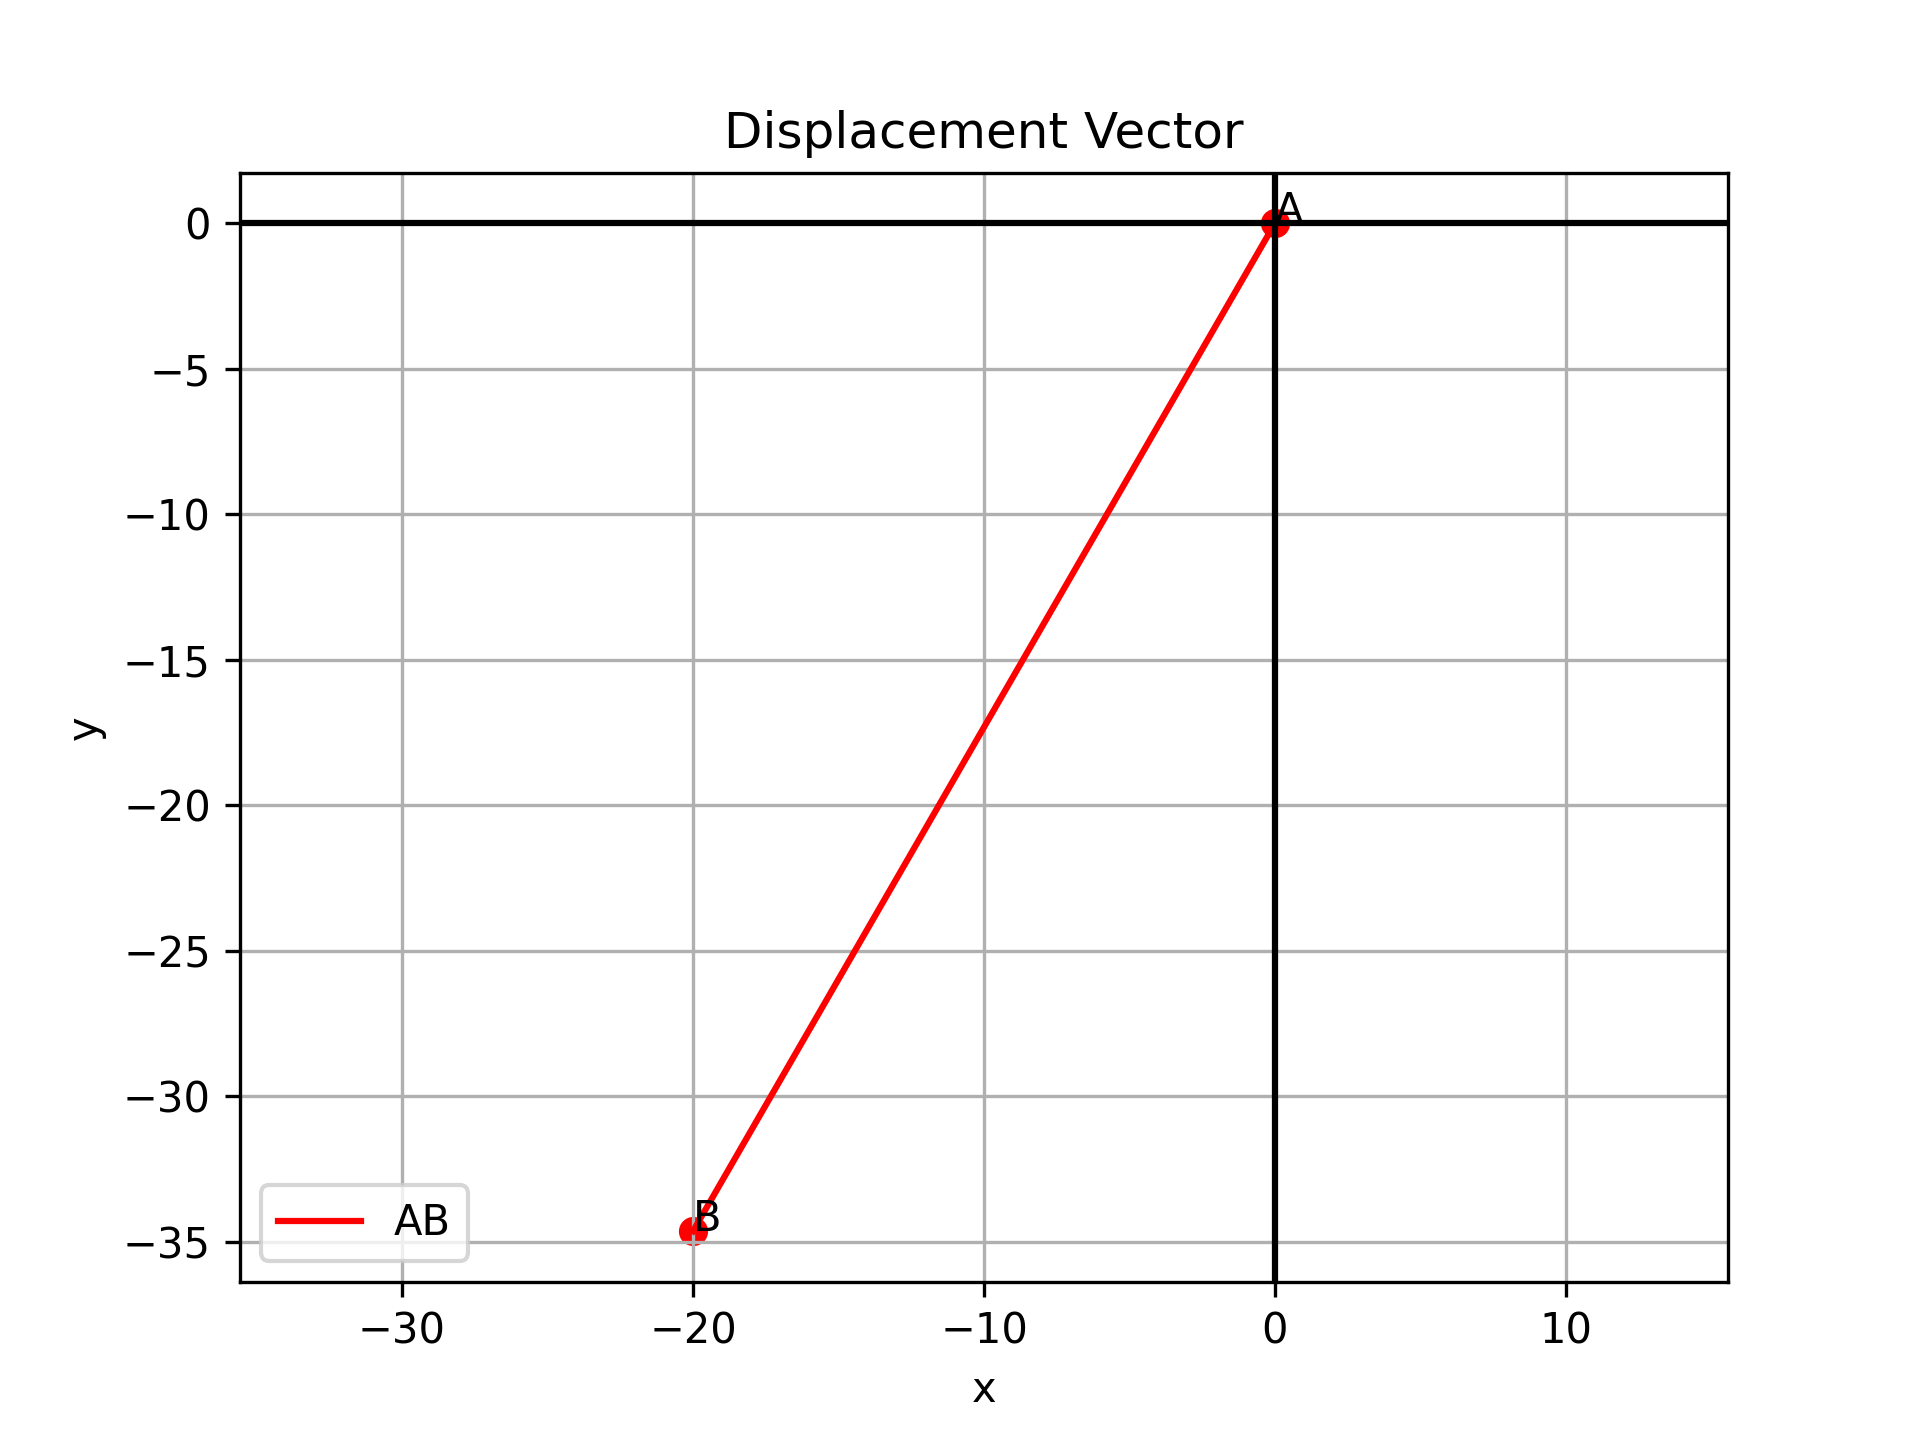
\includegraphics[width=0.65\linewidth]{figs/fig.png}
    \caption{Displacement vector: 40 km, $30^{\circ}$ west of south}
\end{figure}
\end{document}

% \documentclass[journal]{IEEEtran}
% \usepackage[a5paper, margin=10mm, onecolumn]{geometry}
% \usepackage{amsmath, amssymb, mathtools}
% \usepackage{graphicx}
% \usepackage{gvv-book}
% \usepackage{gvv}

% \title{1.2.23 Matgeo}
% \author{ai25btech11015 - M Sai Rithik}

% \begin{document}
% {\let\newpage\relax\maketitle}

% \textbf{Question:} \\
% Represent graphically a displacement of 40 km, $30^{\circ}$ west of south.

% \textbf{Solution:} \\

% We choose the coordinate axes such that:
% \begin{itemize}
%     \item $+x$ axis $\to$ East
%     \item $+y$ axis $\to$ North
% \end{itemize}

% The given displacement has magnitude
% \[
% |\vec{D}| = 40 \ \text{km}
% \]
% and direction $30^{\circ}$ west of south.  

% South corresponds to $270^{\circ}$, hence the angle from the positive $x$-axis is
% \[
% \theta = 270^{\circ} - 30^{\circ} = 240^{\circ}.
% \]

% The vector components are:
% \[
% D_x = 40 \cos 240^{\circ} = -20 \quad , \quad
% D_y = 40 \sin 240^{\circ} = -20\sqrt{3}.
% \]

% Therefore,
% \[
% \vec{D} = -20\hat{i} - 20\sqrt{3}\hat{j}.
% \]

% Thus, the displacement vector is drawn from $(0,0)$ to
% \[
% (-20, \ -20\sqrt{3}).
% \]

% \begin{figure}[h!]
%     \centering
%     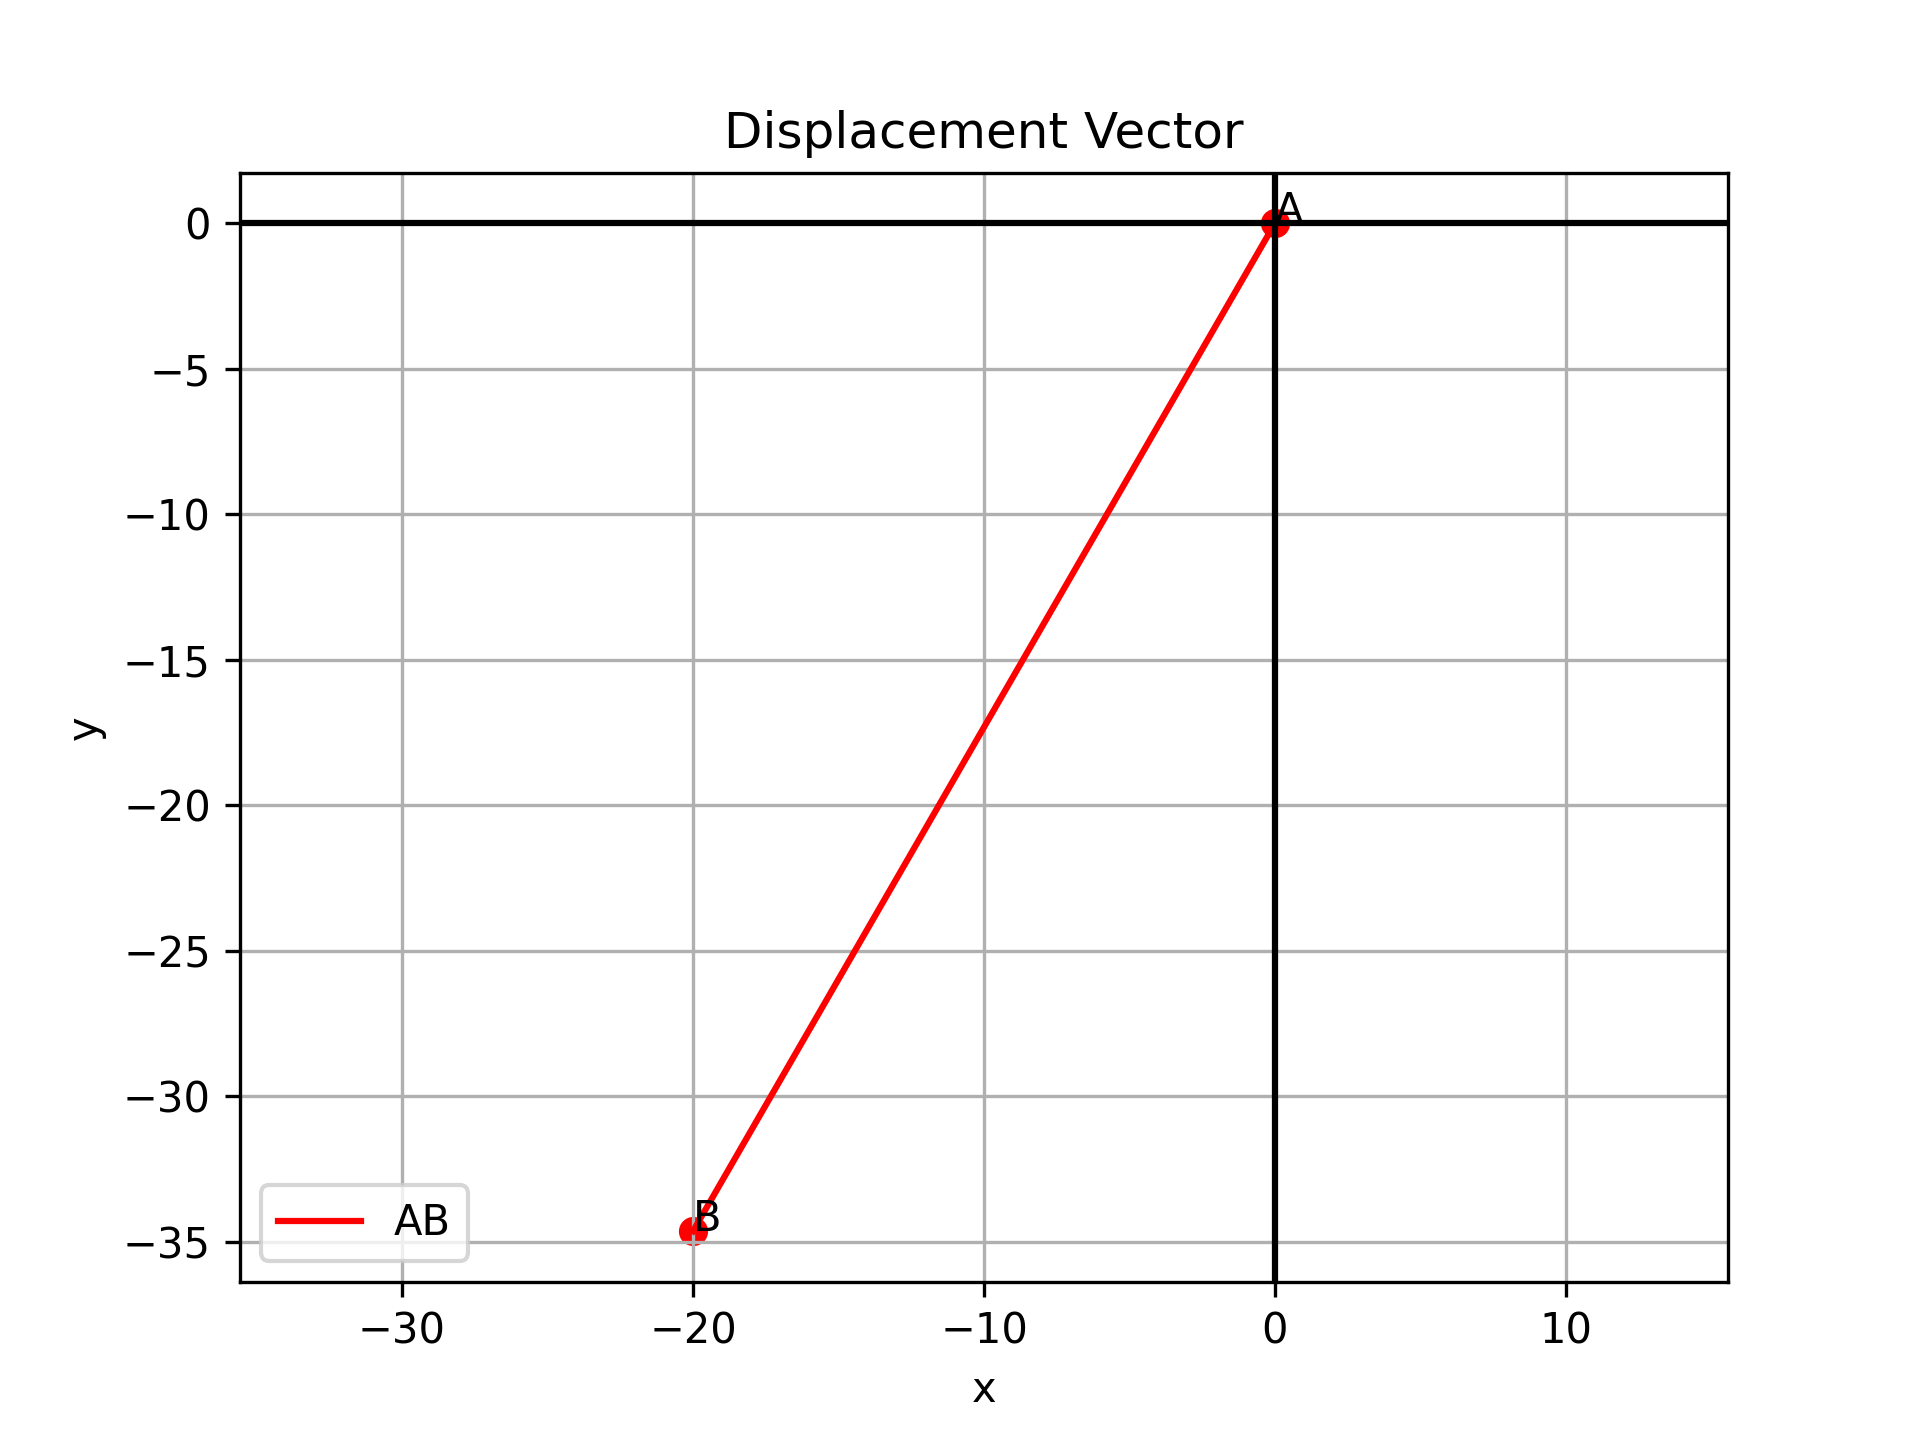
\includegraphics[width=0.65\linewidth]{figs/fig.png}
%     \caption{Displacement vector: 40 km, $30^{\circ}$ west of south}
% \end{figure}

% \end{document}
